\documentclass[11pt]{article}
\usepackage[a4paper,left=27mm,right=27mm,top=27mm,bottom=31mm,footskip=12mm]{geometry}
\usepackage[T1]{fontenc}
\usepackage{lmodern}
\usepackage{microtype}
\usepackage{amsmath,amssymb,amsthm,mathtools}
\usepackage{booktabs,array}
\usepackage{enumitem}
\usepackage{xcolor}
\usepackage{hyperref}
\usepackage{cleveref}
\usepackage{tikz}
\usetikzlibrary{arrows.meta,positioning,decorations.pathmorphing}

\definecolor{deepblue}{HTML}{17365D}
\definecolor{brick}{HTML}{9B2C2C}
\hypersetup{colorlinks=true,linkcolor=deepblue,citecolor=brick,urlcolor=deepblue,
  pdftitle={Cellulation-Independent Boundary Gauge Averaging and Sharp Class-Sector Gaps in 2D Yang--Mills}}

\newtheorem{theorem}{Theorem}[section]
\newtheorem{proposition}[theorem]{Proposition}
\newtheorem{lemma}[theorem]{Lemma}
\newtheorem{corollary}[theorem]{Corollary}
\newtheorem{definition}[theorem]{Definition}
\theoremstyle{remark}
\newtheorem{remark}[theorem]{Remark}
\newtheorem{limitation}[theorem]{Limitation}

\newcommand{\SU}{\mathrm{SU}(2)}
\newcommand{\G}{\mathsf G}
\newcommand{\dd}{\,\mathrm d}
\newcommand{\HclG}{L^2_{\mathrm{cl}}(\G)}
\newcommand{\Pcl}{\mathsf P_{\mathrm{cl}}}
\newcommand{\ip}[2]{\langle #1,#2\rangle}
\DeclareMathOperator{\Tr}{Tr}

\title{\textbf{Cellulation-Independent Boundary Gauge Averaging\\
and Sharp Class-Sector Gaps in Two-Dimensional Yang--Mills}\\[3mm]
\large Compact-group theorem, exact $\mathrm{SU}(2)$ constant, and auditable reduction}
\author{Lluis Eriksson\\
\small with AI-assisted derivation, formalization, and manuscript preparation}
\date{August 2026 \quad Version 0.6}

\begin{document}
\maketitle

\begin{abstract}
Let $\G$ be a compact connected Lie group equipped with a bi-invariant metric.
For two-dimensional $\G$ Yang--Mills with heat-kernel action, we prove a
cellulation-independent finite theorem that turns a framed annular amplitude
into the physical transfer kernel on gauge-invariant boundary states.
An explicit conditional-Haar parametrization makes boundary constraints and
boundary-edge subdivision unambiguous.  Elementary edge and face subdivisions
leave the normalized edge integral unchanged; after a finite subdivision made
only from these two moves, a radial cut exposes one relative
boundary frame, whose normalized Haar average gives
\[
 Z_t(g,h)=\int_{\G}p_t(gxh^{-1}x^{-1})\,\dd x
 =\sum_{\lambda\in\widehat{\G}}e^{-t c_\lambda}
   \chi_\lambda(g)\overline{\chi_\lambda(h)}.
\]
Here $c_\lambda$ is the Casimir eigenvalue.  Thus boundary gauge averaging is
exactly the orthogonal projection of the group heat semigroup onto class
functions.  Writing $c_*(\G)=\min_{\lambda\ne\mathbf1}c_\lambda$, we obtain
reflection positivity, the semigroup law, and the sharp mean-zero norm and gap
\[
 \|T_t\|_{\mathbf1^\perp}=e^{-tc_*(\G)},\qquad
 \operatorname{gap}(T_t)=1-e^{-tc_*(\G)}.
\]
Every irrep of minimum positive Casimir saturates the bound.  For the stated
$\SU$ normalization, $c_*=3/4$, uniquely at the fundamental representation,
so boundary correlations across $k$ equal-area strips decay sharply as
$e^{-3kt/4}$.  We also give a gap calculus for products and finite central
quotients; in particular the induced metric on
$\mathrm{SO}(3)=\SU/\{\pm I\}$ removes the fundamental channel and raises the
minimum from $3/4$ to $2$.  The ingredients are classical; the contribution is their
  quantitative end-to-end assembly, including a tree--cotree disk-elimination
  schedule, subdivision independence, and an explicit machine-checked $\SU$
  frontier.  No claim concerns four-dimensional
Yang--Mills or arbitrary local observables.
\end{abstract}

\noindent\textbf{Keywords.} two-dimensional Yang--Mills; compact Lie group;
heat kernel; subdivision invariance; transfer operator; spectral gap; Lean 4.\\
\textbf{MSC 2020.} 81T13, 81T25, 22E30, 68V20.

\section{Result and epistemic scope}

The character solution and the construction of two-dimensional Yang--Mills on
compact surfaces are classical \cite{Witten1991,Sengupta1997,Levy2003}.  The
point of this paper is not to rediscover them.  It is to state and prove as one
finite quantitative theorem a chain usually split among subdivision moves,
lattice gauge fixing, harmonic analysis, and transfer-operator language:
\begin{center}
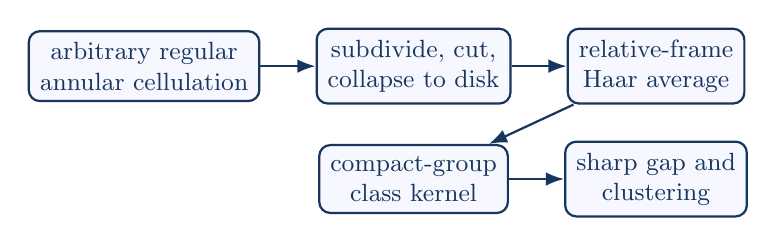
\begin{tikzpicture}[node distance=5mm and 7mm,
  every node/.style={draw,rounded corners,align=center,inner sep=4pt,
    font=\small,fill=blue!3},
  every path/.style={-Latex,thick,deepblue}]
\node (edge) {arbitrary regular\\annular cellulation};
\node[right=of edge] (disk) {subdivide, cut,\\collapse to disk};
\node[right=of disk] (avg) {relative-frame\\Haar average};
\node[below=of disk] (class) {compact-group\\class kernel};
\node[right=of class] (gap) {sharp gap and\\clustering};
\draw (edge)--(disk); \draw (disk)--(avg); \draw (avg)--(class);
\draw (class)--(gap);
\end{tikzpicture}
\end{center}
Each arrow has a different logical status.  All finite-dimensional and
spectral steps are proved below.  The disk edge-integral endpoint and the
concrete $\SU$ character identities have companion Lean proofs.  The topology
is that of a regular finite cellulation of an annulus; no continuum measure,
singular decomposition, or local-field reconstruction is claimed.

Our main result is the following.

\begin{theorem}[Cellulation-independent compact-group transfer]\label{thm:main}
Let $\G$ be a compact connected Lie group with a bi-invariant metric and Haar
measure normalized to one.  Let $t>0$.  On every regular finite annular
cellulation of total area $t$, the heat-kernel lattice amplitude with
gauge-invariant boundary holonomies represented by $g,h\in\G$ is independent
of the cellulation and equals
\begin{equation}\label{eq:class-kernel}
 Z_t(g,h)=\sum_{\lambda\in\widehat{\G}}e^{-tc_\lambda}
 \chi_\lambda(g)\overline{\chi_\lambda(h)}.
\end{equation}
The associated integral operator $T_t$ on $\HclG$ is a positive self-adjoint
contraction satisfying
\[
 T_t\chi_\lambda=e^{-tc_\lambda}\chi_\lambda,\qquad T_sT_t=T_{s+t}.
\]
If $c_*(\G)=\min_{\lambda\ne\mathbf1}c_\lambda$, then on
$\HclG\ominus\mathbb C\mathbf1$,
\begin{equation}\label{eq:sharp-norm}
 \|T_t\|=e^{-tc_*(\G)}.
\end{equation}
Equivalently the bottom of the spectrum of $I-T_t$ on that subspace is
$1-e^{-tc_*(\G)}$.  Equality is attained by every character whose irrep has
Casimir $c_*(\G)$.
\end{theorem}

Compactness and connectedness imply that the Laplacian has discrete spectrum,
the constants are its only zero modes, and $c_*(\G)>0$.  The area $t$ already
includes the coupling and metric convention.  Replacing
the heat generator by $\alpha\Delta$ replaces $t$ everywhere by $\alpha t$.
Stating the convention is essential: numerical gap constants from different
normalizations cannot otherwise be compared.

\section{Compact-group harmonic analysis}

Let $\widehat{\G}$ be the unitary dual.  For $\lambda\in\widehat{\G}$, write
$d_\lambda$, $\chi_\lambda$, and $c_\lambda\ge0$ for its dimension, character,
and Casimir eigenvalue.  Peter--Weyl and elliptic heat-kernel theory give
\begin{equation}\label{eq:full-heat}
 p_t(u)=\sum_{\lambda\in\widehat{\G}}
 d_\lambda e^{-tc_\lambda}\chi_\lambda(u).
\end{equation}
For each fixed $t>0$ the series and all character series used below converge
absolutely and uniformly; this also follows directly from the smoothness of
the heat kernel and standard spectral estimates on a compact manifold.  The
characters form an orthonormal basis of $\HclG$ and satisfy
\begin{equation}\label{eq:orth}
 \int_\G\chi_\lambda(u)\overline{\chi_\mu(u)}\,\dd u
 =\delta_{\lambda\mu},\qquad
 \chi_\lambda(u^{-1})=\overline{\chi_\lambda(u)}.
\end{equation}

The key operation is orbital averaging.

\begin{lemma}[Orbital character product]\label{lem:orbital}
For $a,b\in\G$ and every $\lambda\in\widehat{\G}$,
\begin{equation}\label{eq:orbital}
 \int_\G\chi_\lambda(xax^{-1}b)\,\dd x
 =\frac{\chi_\lambda(a)\chi_\lambda(b)}{d_\lambda}.
\end{equation}
\end{lemma}

\begin{proof}
Let $\rho_\lambda$ be the irreducible unitary representation of dimension
$d_\lambda$.
Schur's lemma applied to
$A=\int_\G\rho_\lambda(x)\rho_\lambda(a)\rho_\lambda(x)^{-1}\,\dd x$
gives $A=(\chi_\lambda(a)/d_\lambda)I$.  Taking the trace after multiplication
by $\rho_\lambda(b)$ proves \eqref{eq:orbital}.
\end{proof}

\begin{remark}
The factor $d_\lambda^{-1}$ in \eqref{eq:orbital} cancels the dimension in
\eqref{eq:full-heat}.  Missing this cancellation is precisely what confuses the
framed heat kernel with the gauge-invariant cylinder kernel.  The conjugating
variable must occur as $xax^{-1}$ in \eqref{eq:orbital}; the superficially
similar word $axa^{-1}$ does not satisfy this identity.
\end{remark}

For $\G=\SU$ with the normalization used in the machine-checked specialization,
irreps are indexed by $n\in\mathbb N_0$ and
\begin{equation}\label{eq:su2-data}
 d_n=n+1,\qquad c_n=\frac{n(n+2)}4,\qquad
 \chi_n(\theta)=\frac{\sin((n+1)\theta)}{\sin\theta}.
\end{equation}
The characters are real and Weyl integration reads
$\int_{\SU}F=(2/\pi)\int_0^\pi F(\theta)\sin^2\theta\,\dd\theta$.

\section{From a physical edge integral to the annulus}

We state the finite model explicitly.  Let $\Gamma$ be an oriented regular
finite cellulation with edge set $E$ and faces $F$.  An edge configuration is
$U\in\G^E$.  If $U_f$ is the ordered face holonomy and $a_f>0$ its area, the
heat-kernel density is
\begin{equation}\label{eq:edge-density}
 \rho_\Gamma(U)=\prod_{f\in F}p_{a_f}(U_f),\qquad
 t=\sum_{f\in F}a_f.
\end{equation}
All edge integrations use product probability Haar measure.  There is no
formal path integral in this definition.

\begin{definition}[Boundary-conditioned amplitude]\label{def:amplitude}
Choose one marked vertex on each boundary and fix representatives $g,h\in\G$
of the two oriented boundary holonomies.  Reorient the edges of an oriented
boundary cycle in its direction and write them as $b=(e_1,\ldots,e_r)$ from
the marked vertex.  Its conditional Haar integral at holonomy $g$ is
\begin{equation}\label{eq:conditional-haar}
 \int_{\operatorname{Hol}_b=g}\!\Phi\,\dd\nu_g
 :=\int_{\G^{r-1}}
 \Phi\!\left(u_1,\ldots,u_{r-1},
 (u_1\cdots u_{r-1})^{-1}g\right)
 \prod_{j=1}^{r-1}\dd u_j .
\end{equation}
If the ambient orientation gives an inverse edge, the corresponding coordinate
is inverted; inversion preserves Haar probability.  The amplitude
$Z_\Gamma(g,h)$ is the integral of \eqref{eq:edge-density} against product Haar
on internal edges and the two measures \eqref{eq:conditional-haar}.  Thus no
delta distribution or omitted gauge-volume normalization is hidden in the
notation.  Independent changes of frame at the two marked vertices conjugate
$g$ and $h$, so the physical amplitude is a class function in each variable.
\end{definition}

\begin{lemma}[Canonical boundary fibre]\label{lem:boundary-fibre}
The value in \eqref{eq:conditional-haar} is independent of which boundary edge
is solved for.  If a boundary edge is replaced by two consecutive edges, the
multiplication map from their conditional Haar coordinates to the old edge
coordinate pushes the new fibre measure to the old one.
\end{lemma}

\begin{proof}
It suffices to compare adjacent eliminated coordinates.  Freeze every other
edge, absorb their ordered product and $g$ into a fixed $C\in\G$, and call the
two adjacent coordinates $v,y$.  The constraint has the form $vy=C$.  Solving
for $v$ parametrizes the fibre by $y\mapsto(Cy^{-1},y)$; solving for $y$
parametrizes it by $v\mapsto(v,v^{-1}C)$.  The transition $y\mapsto Cy^{-1}$
is an inversion followed by a translation and hence preserves normalized Haar
measure.  Adjacent exchanges connect all choices.

For a subdivision write the old coordinate as $u=ab$.  Haar invariance gives
\[
 \int_{\G^2}F(ab)\,\dd a\dd b=\int_\G F(u)\,\dd u.
\]
On a fixed-holonomy fibre,
one of $a,b$ is solved from the same ordered-product constraint; the remaining
coordinate integrates to one.  This proves the stated pushforward, including
the case in which the old edge was the eliminated coordinate.
\end{proof}

The next lemma is the finite mechanism behind cellulation independence.

\begin{lemma}[Exact elementary subdivision moves]\label{lem:subdivision}
The boundary-conditioned amplitude is unchanged by either of the following
moves, with the boundary data held fixed:
\begin{enumerate}[label=(\roman*),nosep]
\item subdivision of an edge into two consecutive edges;
\item subdivision of a face of area $a+b$ by a new edge into faces of positive
areas $a$ and $b$.
\end{enumerate}
Consequently it is unchanged under any finite sequence of such subdivisions
or their inverses whenever the inverse cellulation remains regular.
\end{lemma}

\begin{proof}
For (i), every occurrence of the old variable $u$ is replaced by $u_1u_2$.
For any integrable $F$, Haar invariance and normalization give
\[
 \int_{\G^2}F(u_1u_2)\,\dd u_1\dd u_2=\int_\G F(u)\,\dd u.
\]
The extra vertex therefore contributes exactly one, not a gauge-volume factor.
If the edge is on a conditioned boundary, the same conclusion is precisely
the fibre-pushforward statement of \cref{lem:boundary-fibre}; hence this proof
does not silently exclude subdivision of the edge used to impose holonomy.
For (ii), orient the new edge so that the two new face words are $Au$ and
$u^{-1}B$.  The heat-semigroup convolution identity gives
\[
 \int_\G p_a(Au)p_b(u^{-1}B)\,\dd u=p_{a+b}(AB),
\]
which is precisely the old face factor.  Fubini proves both statements inside
the full edge integral.
\end{proof}

\begin{lemma}[A radial cut after finite subdivision]\label{lem:topological-cut}
Every regular finite cellulation of an annulus has a finite regular subdivision
whose one-skeleton contains a simple path joining the two boundary components.
Cutting along this path produces a disk cellulation; its exterior word consists
of the first physical boundary, one copy of the path, the oppositely oriented
second boundary, and the reverse copy of the path.
\end{lemma}

\begin{proof}
Choose a properly embedded PL arc $\alpha$ between the boundary components and
put it in general position with respect to the original one-skeleton: its
endpoints lie in boundary edges, it avoids old vertices, and its finitely many
interior intersections with edges are transverse.  First subdivide every edge
at an intersection point (and at the two endpoints).  These are moves (i) of
\cref{lem:subdivision}.  In each old face the components of $\alpha$ are now
pairwise disjoint polygonal arcs with endpoints at vertices of the subdivided
boundary.  Insert these arcs one at a time.  Each insertion divides one disk
face into two disk faces, so it is move (ii); choose positive daughter areas
whose sum is the old face area.  After finitely many insertions $\alpha$ is a
simple edge path in the new regular cellulation.  This gives directly the
required subdivision using only the two analytically invariant moves, rather
than appealing to an unmatched stellar operation.  Cutting an annulus along a
proper boundary-to-boundary arc produces a disk, and its oriented boundary is
the first physical boundary, one copy of $\alpha$, the oppositely oriented
second boundary, and the reverse copy of $\alpha$.
\end{proof}

Let $D$ be the disk obtained from the chosen cut.  We write $A_D(q)$ for its
conditioned edge integral with exterior holonomy fixed to $q\in\G$; all other
edge variables are integrated against product Haar probability.

\begin{lemma}[Exact disk collapse]\label{lem:disk-collapse}
For every regular disk cellulation with positive face areas $a_f$ and exterior
holonomy $q$,
\begin{equation}\label{eq:disk-collapse}
 A_D(q)=p_{\sum_f a_f}(q).
\end{equation}
\end{lemma}

\begin{proof}
Choose the boundary edge eliminated by \eqref{eq:conditional-haar} and call it
$e_0$.  The remaining boundary edges form a path, so they extend to a primal
spanning tree $T$ containing every boundary edge except $e_0$.  Root $T$ at the
marked boundary vertex.  Successively changing from a tree-edge variable to
the group element at its child vertex is triangular: every step is a left or
right Haar translation.  Gauge covariance of face holonomy and centrality of
$p_{a_f}$ then set every tree edge to the identity, with each tree-coordinate
integral contributing exactly one.

Euler's identity $|E|-|V|+1=|F|$ leaves one chord per bounded face.  Elementary
planar tree--cotree duality says that the duals of $E\setminus T$ form a tree on
the bounded faces and the exterior face.  Because $T$ contains all boundary
edges except $e_0$, the dual of $e_0$ is its unique edge incident to the
exterior.  Remove that dual edge and root the resulting tree of bounded faces
at the face adjacent to $e_0$.

Now eliminate bounded faces from the leaves toward the root.  For a non-root
leaf, its parent chord occurs once in its face word and once with opposite
orientation in the parent word.  After absorbing the other fixed factors into
$A,B\in\G$, the relevant integral is exactly
\[
 \int_\G p_a(Au)p_b(u^{-1}B)\,\dd u=p_{a+b}(AB).
\]
Thus integrating the parent chord deletes that leaf and merges its positive
area into the parent.  This is a finite, explicitly ordered elimination; it
continues until one face remains.  Its boundary word is the fixed exterior
holonomy $q$ and its area is $\sum_fa_f$, proving \eqref{eq:disk-collapse}.
The argument uses only normalized Haar invariance, centrality, planar
tree--cotree duality, and heat-kernel convolution, and is valid for every
compact group in the hypotheses.
\end{proof}

\begin{lemma}[Radial-cut disintegration]\label{lem:cut-disintegration}
For a subdivided annular cellulation as in \cref{lem:topological-cut} and fixed
oriented boundary holonomies
$g,h$, cutting and regluing give the exact finite-dimensional identity
\begin{equation}\label{eq:cut-disintegration}
 Z_\Gamma(g,h)=\int_G A_D(gxh^{-1}x^{-1})\,\dd x.
\end{equation}
No heat-kernel expansion is used in this step.
\end{lemma}

\begin{proof}
The boundary representatives $g$ and $h$ are held fixed throughout; only
internal coordinates are changed.  Orient the two copies of the cut oppositely
and choose a rooted spanning tree
of the cut-open disk containing all but one of the cut-path links.  Introduce
a vertex potential $k_v\in\G$ recursively along the tree and replace every
edge variable by
\[
 U_e\longmapsto k_{s(e)}^{-1}U_e k_{t(e)}.
\]
For fixed values of the other coordinates this is a composition of left and
right translations on $\G$; normalized Haar measure is therefore unchanged.
Every tree edge becomes the identity.  Centrality of each $p_{a_f}$ makes every
face factor invariant under the simultaneous vertex conjugations, so no
Jacobian or residual vertex-volume factor appears.

No boundary representative is integrated and no boundary gauge is divided out
in this coordinate change.  The only coordinate not removed by the internal
tree gauge is the transport $x$ from
the frame of the first boundary to that of the second.  Reading the exterior
word of the disk from the first boundary, the four surviving blocks are
$g$, $x$, $h^{-1}$, and $x^{-1}$, in that order.  Thus the conditional integral
at fixed $x$ is $A_D(gxh^{-1}x^{-1})$.  Regluing identifies the two copies of
the cut but does not fix their relative frame; Fubini disintegrates the product
Haar integral over this last coordinate.  Integrating $x$ proves
\eqref{eq:cut-disintegration}.
\end{proof}

\begin{proposition}[Cellulation-independent annular reduction]\label{prop:cut-glue}
For every regular finite annular cellulation of total area $t$,
\begin{equation}\label{eq:orbit-heat}
 Z_t(g,h)=\int_G p_t(gxh^{-1}x^{-1})\,\dd x.
\end{equation}
\end{proposition}

\begin{proof}
Use \cref{lem:topological-cut} to choose a finite subdivision containing a
radial edge path.  By \cref{lem:subdivision}, the original and subdivided
boundary amplitudes are identical.  The fixed-boundary disk theorem gives
$A_D(q)=p_t(q)$ by the explicit tree--cotree schedule in
\cref{lem:disk-collapse}; no gauge-fixing or face-elimination choice is left
implicit.
Substitute this disk identity into \eqref{eq:cut-disintegration}.  The resulting
right side depends only on $t,g,h$, proving cellulation independence as well.
\end{proof}

\begin{figure}[t]
\centering
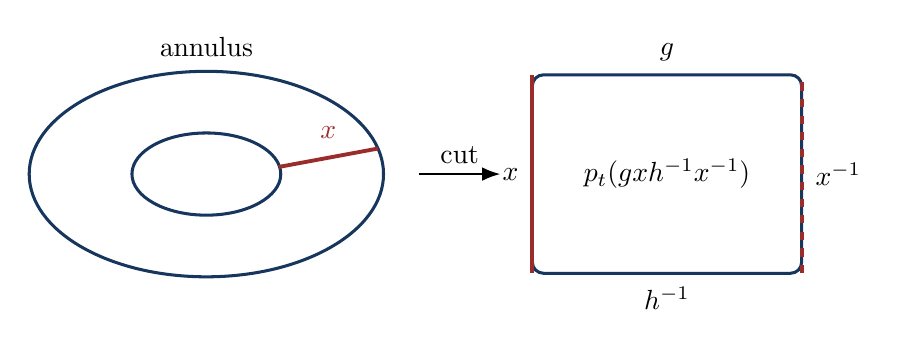
\begin{tikzpicture}[>=Latex,thick,scale=.9]
  \draw[deepblue,line width=1.1pt] (0,0) ellipse (2.5 and 1.45);
  \draw[deepblue,line width=1.1pt] (0,0) ellipse (1.05 and .58);
  \draw[brick,line width=1.4pt] (1.02,.10) -- (2.42,.36);
  \node[brick,above] at (1.72,.35) {$x$};
  \node at (0,1.8) {annulus};
  \draw[->] (3.0,0) -- (4.15,0) node[midway,above]{cut};
  \draw[deepblue,line width=1.1pt,rounded corners] (4.6,-1.4) rectangle (8.4,1.4);
  \draw[brick,line width=1.4pt] (4.6,-1.4)--(4.6,1.4);
  \draw[brick,line width=1.4pt,dashed] (8.4,-1.4)--(8.4,1.4);
  \node[left] at (4.55,0) {$x$};
  \node[right] at (8.45,0) {$x^{-1}$};
  \node[above] at (6.5,1.45) {$g$};
  \node[below] at (6.5,-1.45) {$h^{-1}$};
  \node at (6.5,0) {$p_t(gxh^{-1}x^{-1})$};
\end{tikzpicture}
\caption{A radial cut exposes a relative boundary frame $x$.  The disk edge
integral collapses to one heat kernel; gluing Haar-averages $x$.}
\label{fig:cut}
\end{figure}

\begin{theorem}[Boundary gauge projection]\label{thm:projection}
For $t>0$ and $g,h\in\G$,
\begin{equation}\label{eq:projection}
 \int_\G p_t(gxh^{-1}x^{-1})\,\dd x
 =\sum_{\lambda\in\widehat{\G}}e^{-tc_\lambda}
 \chi_\lambda(g)\overline{\chi_\lambda(h)}.
\end{equation}
The series converges absolutely and uniformly on $\G\times\G$ for fixed
$t>0$.
\end{theorem}

\begin{proof}
Absolute uniform convergence of the heat-kernel character expansion justifies
termwise integration.  Insert \eqref{eq:full-heat}, cyclically permute inside
the character, and apply \cref{lem:orbital} with $a=h^{-1}$ and $b=g$.
Then $\chi_\lambda(h^{-1})=\overline{\chi_\lambda(h)}$, and the orbital factor
$d_\lambda^{-1}$ cancels the dimension in \eqref{eq:full-heat}.  Uniform
convergence of the resulting series follows from
$|\chi_\lambda|\le d_\lambda$ and
$\sum_\lambda d_\lambda^2e^{-tc_\lambda}<\infty$, the heat trace of the
scalar Laplacian on the compact manifold $\G$.
\end{proof}

\begin{remark}[Framed versus gauge-invariant boundaries]
The framed transition density is $p_t(gh^{-1})$ on $L^2(\G)$ and contains all
matrix coefficients.  The kernel $Z_t$ in \eqref{eq:projection} acts on
$\HclG$ and contains one character per irreducible representation.  They are
related by orthogonal projection, but are not pointwise equal.
\end{remark}

\section{Transfer operator and reflection positivity}

Define conjugation averaging on $L^2(\G)$ by
\begin{equation}\label{eq:class-projection}
 (\Pcl f)(g)=\int_\G f(xgx^{-1})\,\dd x.
\end{equation}

\begin{proposition}[Boundary averaging is an orthogonal projection]
\label{prop:conditional-expectation}
The operator $\Pcl$ is a self-adjoint idempotent contraction whose range is
exactly $\HclG$.  It preserves constants and positivity.  If $S_t$ is the full
group heat semigroup with kernel $p_t(gh^{-1})$, then
\begin{equation}\label{eq:commuting-square}
 \Pcl S_t=S_t\Pcl,\qquad
 T_t=S_t|_{\HclG}=\Pcl S_t\Pcl|_{\HclG}.
\end{equation}
Thus the physical cylinder operator is a genuine invariant-sector restriction,
not an unrelated kernel obtained by deleting dimension factors by hand.
\end{proposition}

\begin{proof}
Haar invariance gives $\Pcl^2=\Pcl$: after two averages, replace the second
conjugating variable $y$ by $yx^{-1}$.  The same changes of variables show
$\ip{\Pcl f}{g}=\ip{f}{\Pcl g}$, so an idempotent $\Pcl$ is the orthogonal
projection onto its range.  Its fixed points are precisely the conjugation-
invariant functions.  Averaging preserves $1$, nonnegativity, and the
$L^2$ norm bound by Jensen's inequality.  Finally, $p_t$ is central, so
conjugation commutes with convolution by $p_t$.  Restricting the resulting
commuting square to the fixed-point space gives \eqref{eq:commuting-square};
its two-point kernel is \eqref{eq:projection}.
\end{proof}

Define, initially on continuous class functions,
\begin{equation}\label{eq:transfer}
 (T_tf)(g)=\int_\G Z_t(g,h)f(h)\,\dd h.
\end{equation}
Uniform convergence and \eqref{eq:orth} give the diagonal action
\begin{equation}\label{eq:diagonal}
 T_t\chi_\lambda=e^{-tc_\lambda}\chi_\lambda.
\end{equation}
It follows immediately that $T_t$ extends to a positive self-adjoint
contraction on $\HclG$, $T_t\mathbf1=\mathbf1$, and $T_sT_t=T_{s+t}$.

\begin{proposition}[Reflection form]\label{prop:rp}
For $s>0$ and $F\in\HclG$,
\begin{equation}\label{eq:rp}
 \iint_{\G\times\G}\overline{F(g)}Z_{2s}(g,h)F(h)\,\dd g\dd h
 =\|T_sF\|_2^2\ge0.
\end{equation}
For a finite family $F_j\in\HclG$ and coefficients $z_j\in\mathbb C$, the
corresponding matrix of reflected pairings is positive semidefinite.
\end{proposition}

\begin{proof}
The semigroup identity gives
$Z_{2s}(g,h)=\int_GZ_s(g,k)Z_s(k,h)\,\dd k$.  Fubini and self-adjointness turn
the left side into $\int_\G|(T_sF)(k)|^2\,\dd k$.  Replace $F$ by
$\sum_jz_jF_j$ for the matrix statement.
\end{proof}

This is the transfer-kernel form of Osterwalder--Schrader positivity for the
one-dimensional time slicing supplied by the cylinder.  We do not claim here
a reconstruction of a local two-dimensional Wightman field theory; the
bounded transfer operator is the precise object proved positive.

\section{Exact compact-group gap and sharp boundary clustering}

Let $\HclG^0=\{f\in\HclG:\int_\G f=0\}$.  The trivial character is
$\mathbf1$, so $\HclG^0$ is the closed span of the nontrivial irreducible
characters.  Since $\G$ is connected and the metric is positive definite,
the scalar Laplacian has constants as its entire kernel.  Discreteness of its
spectrum therefore gives
\[
 c_*(\G):=\min_{\lambda\ne\mathbf1}c_\lambda>0.
\]

\begin{theorem}[Sharp compact-group mean-zero norm]\label{thm:gap}
For $t>0$,
\[
 \|T_t|_{\HclG^0}\|=e^{-tc_*(\G)},\qquad
 \inf\sigma\bigl((I-T_t)|_{\HclG^0}\bigr)=1-e^{-tc_*(\G)}.
\]
The equality space is exactly the span of characters with
$c_\lambda=c_*(\G)$.
\end{theorem}

\begin{proof}
Write $f=\sum_{\lambda\ne\mathbf1}a_\lambda\chi_\lambda$.  Parseval and
\eqref{eq:diagonal} give
\[
 \|T_tf\|_2^2
 =\sum_{\lambda\ne\mathbf1}e^{-2tc_\lambda}|a_\lambda|^2
 \le e^{-2tc_*(\G)}\sum_{\lambda\ne\mathbf1}|a_\lambda|^2.
\]
Any character with minimum positive Casimir attains equality.  The equality
condition in the weighted sum also identifies the entire equality space.  The
spectral statement for $I-T_t$ follows from the same diagonalization.
\end{proof}

\begin{corollary}[Sharp boundary strip clustering]\label{cor:clustering}
Let $f,g\in\HclG^0$ and let $k\ge0$ be an integer.  Across $k$ strips of area
$t>0$,
\begin{equation}\label{eq:cluster}
 |\ip{f}{T_t^kg}|\le e^{-ktc_*(\G)}\|f\|_2\|g\|_2.
\end{equation}
The exponential rate and prefactor-one operator bound are sharp.  Equality is
obtained by taking $f=g$ to be any unit character of minimum positive Casimir.
\end{corollary}

\begin{proof}
$T_t^k=T_{kt}$ and \cref{thm:gap} give the bound by Cauchy--Schwarz; a minimum-
Casimir character gives equality.
\end{proof}

\begin{corollary}[Exact $\SU$ constant]\label{cor:su2}
For $\G=\SU$ with \eqref{eq:su2-data},
\[
 c_*(\SU)=\frac34,\qquad
 \|T_t|_{\mathbf1^\perp}\|=e^{-3t/4},\qquad
 \operatorname{gap}(T_t)=1-e^{-3t/4}.
\]
The minimum is unique and the equality space is $\mathbb C\chi_1$.  Hence
\eqref{eq:cluster} becomes the sharp bound $e^{-3kt/4}$.
\end{corollary}

\begin{proof}
For $n\ge1$, \eqref{eq:su2-data} and
$n(n+2)-3=(n-1)(n+3)\ge0$ show that $c_n\ge3/4$, with equality only at $n=1$.
Apply \cref{thm:gap,cor:clustering}.
\end{proof}

The compact-group formulation reveals how the boundary gap changes under two
basic operations.  This is sometimes hidden when one works only with a fixed
matrix group.

\begin{proposition}[Product and central-quotient gap calculus]
\label{prop:gap-calculus}
Let $\G_1,\G_2$ carry product-normalized bi-invariant metrics.
\begin{enumerate}[label=(\roman*),itemsep=2pt]
\item For the product metric,
\[
 c_*(\G_1\times\G_2)=\min\{c_*(\G_1),c_*(\G_2)\}.
\]
If the first minimum is smaller, the minimum sector is the first minimum sector
tensored with the trivial representation of the second; the symmetric statement
holds if the second is smaller.  If they coincide, the two families form the
minimum sector.
\item If $\Gamma$ is a finite central subgroup of $\G$ and $\G/\Gamma$ has the
induced quotient metric, then
\[
 c_*(\G/\Gamma)
 =\min_{\substack{\lambda\ne\mathbf1\\ \Gamma\subseteq\ker\rho_\lambda}}
 c_\lambda\ \ge\ c_*(\G).
\]
The inequality is strict exactly when no minimum-Casimir irrep of $\G$ is
trivial on $\Gamma$.
\end{enumerate}
Consequently, in the normalization \eqref{eq:su2-data},
\begin{equation}\label{eq:so3-gap}
 c_*(\mathrm{SO}(3))=2,\qquad
 \operatorname{gap}(T_t^{\mathrm{SO}(3)})=1-e^{-2t}.
\end{equation}
\end{proposition}

\begin{proof}
Every irrep of a product is $\lambda_1\boxtimes\lambda_2$, and the product
Laplacian gives $c_{\lambda_1\boxtimes\lambda_2}=c_{\lambda_1}+c_{\lambda_2}$.
The smallest nonzero sum is therefore the smaller factor minimum, with the
stated equality sector.  Irreps of $\G/\Gamma$ are exactly the irreps of $\G$
whose kernels contain $\Gamma$.  The quotient map is a local isometry, so their
Casimir eigenvalues are unchanged.  Taking the minimum over this restricted
dual proves (ii) and its strictness criterion.  For
$\SU/\{\pm I\}$, precisely the even labels $n$ descend.  The first nontrivial
one is $n=2$, and \eqref{eq:su2-data} gives $c_2=2$.
\end{proof}

\begin{remark}[Generator gap]
The generator $H$ defined spectrally by
$H\chi_\lambda=c_\lambda\chi_\lambda$ is unbounded, but
$T_t=e^{-tH}$ is bounded.  Its lowest nonzero energy is $c_*(\G)$, equal to
$3/4$ in the stated $\SU$ normalization.  The bounded
statement \eqref{eq:sharp-norm}, specialized to $\SU$, is what the current
formal interface certifies.  Calling
this the solution of the four-dimensional Yang--Mills mass-gap problem would
be false: the dimension, dynamics, and target theorem are different.
\end{remark}

\section{What is machine checked}

The companion Lean development uses Mathlib's concrete $\SU$, constructs
normalized Haar probability, proves the Weyl character formulas and their
orthogonality, and proves the actual infinite heat-kernel convolution
semigroup.  The following endpoints are directly relevant:
\begin{center}
\begin{tabular}{>{\raggedright\arraybackslash}p{.43\textwidth}
                >{\raggedright\arraybackslash}p{.47\textwidth}}
\toprule
Lean endpoint & Mathematical content\\
\midrule
\nolinkurl{integral_su2Haar_orbit_character_general}
  & orbital product formula \eqref{eq:orbital}\\
\nolinkurl{integral_su2ClassHeatKernel_mul}
  & infinite class-kernel semigroup with a genuine Haar integral\\
\nolinkurl{su2Migdal_twoFace_class_merge}
  & two-face class Migdal merge\\
\nolinkurl{conditionedEdgeModelAmplitude_eq_heatKernel}
  & fixed-boundary physical disk edge integral equals the heat kernel\\
\nolinkurl{su2ClassTransferMultiplier_le_fundamental}
  & every non-vacuum multiplier is bounded by $e^{-3t/4}$\\
\nolinkurl{su2ClassTransferMultiplier_bound_sharp}
  & the fundamental mode attains that bound\\
\bottomrule
\end{tabular}
\end{center}

The fixed-boundary disk theorem lives on the
\href{https://github.com/lluiseriksson/lean-2d-yang-mills/tree/agent/su2-boundary-conditioned-bridge}{public boundary-conditioned branch} at commit
\texttt{6dbb8cebc18ab2d65b6ae24af5216347c476df3f}; its provenance file identifies
the audited mathematical snapshot
\texttt{a1fbea97cbe673d383dbb4bc5e2a2fb70dbf190a}.  The sharp multiplier lemmas are
included with this manuscript as \texttt{SU2ClassTransferGap.lean}.
The exact target \texttt{Lean2dYangMills.SU2ClassTransferGap} was rebuilt in
this environment from the pinned manifest: Lake completed all 2,817 jobs with
exit code zero.  A separate \texttt{\#print axioms} audit reports only
\texttt{propext}, \texttt{Classical.choice}, and \texttt{Quot.sound} for the
four new endpoints.  The exact boundary-conditioned commit was also rebuilt as
the complete \texttt{Lean2dYangMills} library: Lake completed all 3,097 jobs
with exit code zero, including the physical disk endpoint cited above.

\begin{limitation}[Formalization boundary]
The current Lean corpus does not yet package elementary subdivision invariance,
the PL radial-cut reduction, and the disk collapse as one theorem about regular
annular combinatorial maps, nor does it
construct the $L^2$ completion and its unbounded generator.  Accordingly, the
machine-checked claim is the conjunction of the disk integral, orbital
character identity, class semigroup, and scalar sharp multiplier bound.  The
compact-group extension, topological reduction, and Hilbert-space assembly are
proved in this paper, but are not advertised as one monolithic Lean theorem.
\end{limitation}

\section{Reproducibility and falsification checks}

The deterministic script \texttt{repro/replay.py} performs five diagnostics:
\begin{enumerate}
\item the removable endpoint values
$\chi_n(0)=n+1$ and $\chi_n(\pi)=(-1)^n(n+1)$ are tested exactly;
\item Gauss--Legendre integration of the Weyl formula checks the character
Gram matrix;
\item multiplier arithmetic checks $e^{-sc_n}e^{-tc_n}=e^{-(s+t)c_n}$;
\item a finite spectral search checks that $n=1$ is the unique sharp mode;
\item a random complex character polynomial checks positivity of the reflected
quadratic form.
\end{enumerate}
These floating-point checks are useful falsifiers for normalization and sign
errors, but they are not substitutes for proof.  A successful run prints
\texttt{REPLAY: PASS}.

\section{Novelty, priority, and limitations}

Migdal's lattice solution, the heat-kernel formulation, and Witten's character
expansion make the basic cylinder formula classical
\cite{Migdal1975,Witten1991,Levy2003}.  The Markov/gluing structure of the
rigorous two-dimensional Yang--Mills measure is also established in the
literature \cite{Levy2003,DriverGabrielHallKemp2017}.  We therefore make no
priority claim for \eqref{eq:class-kernel} or for diagonalizing a compact-group
heat semigroup.

The present theorem is therefore an assembly result, not a priority claim for
the character solution or for subdivision invariance separately.  Its
increment through Version 0.5 is mathematically explicit: the restriction to an
``admissible'' $\SU$ cellulation has been removed, and the sharp spectral
statement is parametrized by the minimum positive Casimir of an arbitrary
compact connected structure group.  The contribution claimed here is:\par
\begin{itemize}[leftmargin=7mm,topsep=4pt,itemsep=3pt]
\item an explicit finite-edge-to-transfer chain with all normalization factors;
\item exact invariance under the two elementary subdivision moves and a finite
PL reduction from every regular annular cellulation to a radial-cut model;
\item a theorem-level distinction between framed and gauge-invariant boundary
kernels;
\item the exact compact-group transfer gap $1-e^{-tc_*(\G)}$ and sharp boundary
strip-clustering constant in the same convention as the physical edge integral;
\item a precise map of which links are already machine checked and which are
paper proofs.
\end{itemize}

Version 0.6 does not enlarge that novelty claim.  It closes three proof
interfaces that were previously compressed: the conditional Haar measure is
given by coordinates and shown independent of the eliminated boundary edge;
the PL arc is inserted using exactly the edge and face moves covered by the
analytic invariance lemma; and the disk identity is proved by a finite
tree--cotree elimination schedule.  These changes strengthen self-containment
and falsifiability, not historical priority.

The result is special to the exactly soluble two-dimensional heat-kernel model.
It does not address four-dimensional continuum Yang--Mills, interacting local
observables in four dimensions, or the Clay Millennium problem.  Nor does it
turn the boundary estimate into clustering for arbitrary local bulk observables
or an Osterwalder--Schrader reconstruction.  Regular finite cellulations are
covered; singular CW decompositions and continuum limits are not.

\section{Conclusion}

Two elementary Haar identities make the finite annular theory independent of
its regular cellulation; a radial cut then exposes boundary gauge averaging as
the hinge between the physical edge model and the class-function transfer
operator.  The dimension factor cancels for every compact connected $\G$,
reflection positivity is a semigroup square, and the sharp gap is fixed by
$c_*(\G)$.  For $\SU$ the unique fundamental channel saturates the exact
$e^{-3t/4}$ decay.  The theorem remains deliberately modest about priority and
dimension, but the normalization, cellulation reduction, physical integral,
spectral optimum, and formal frontier now belong to one checkable chain.

\appendix
\section{Coefficient-level proof of positivity}

For a finite character polynomial
$F=\sum_{\lambda\in\Lambda}a_\lambda\chi_\lambda$, direct insertion
into \eqref{eq:rp} gives
\[
 \iint\overline{F(g)}Z_{2s}(g,h)F(h)\,\dd g\dd h
 =\sum_{\lambda\in\Lambda}e^{-2sc_\lambda}|a_\lambda|^2.
\]
This formula simultaneously proves positivity and locates its null space.  At
positive time every coefficient is strictly positive, so the reflected form is
strictly positive on nonzero finite character polynomials.  Density extends it
to all of $\HclG$; strict positivity remains, although there is no uniform
lower bound because the Casimir spectrum is unbounded.

\section{SU(2) normalization cross-check}

At $n=0$, $c_0=0$ and $T_t\mathbf1=\mathbf1$.  At $n=1$,
$c_1=3/4$.  At $n=2$, $c_2=2$.  Hence the first multipliers are
\[
 1,\quad e^{-3t/4},\quad e^{-2t},\quad e^{-15t/4},\ldots.
\]
The full heat kernel at the identity begins instead as
\[
 p_t(1)=1+4e^{-3t/4}+9e^{-2t}+16e^{-15t/4}+\cdots,
\]
because $p_t(1)$ contains $d_n\chi_n(1)=d_n^2$.  The two-point class kernel at
$(1,1)$ has the same diagonal value, while its expansion at general $(g,h)$ has
no dimension coefficient.  This is a compact check that all three formulas are
consistent rather than interchangeable.

\section{Exact reproduction protocol}

The single release archive contains the manuscript and its complete audit
payload.  At its root are \texttt{paper.pdf}, \texttt{manuscript.tex},
\texttt{RELEASE\_NOTES.md}, and \texttt{MANIFEST.sha256}.  Its
\texttt{repro/} directory contains:
\begin{itemize}[leftmargin=8mm,nosep]
\item \texttt{replay.py};
\item \texttt{SU2ClassTransferGap.lean};
\item \texttt{AuditClassTransferGap.lean};
\item \texttt{requirements.txt} and a command-level \texttt{README.md};
\item \texttt{reproduce.ps1};
\item \texttt{lean-2d-yang-mills.bundle}, a complete Git history containing
both exact cited commits;
\item \texttt{pinned-main/}, containing the main commit's exact Lake manifest,
package file, and Lean toolchain declaration.
\end{itemize}
Thus neither the PDF nor the Lean dependency snapshot has to be obtained as a
second attachment.  Every preserved file is covered by the root manifest.
From \texttt{repro/}, the numerical replay alone is
\begin{verbatim}
python -m pip install -r requirements.txt
python replay.py
\end{verbatim}
and the complete two-checkout Lean replay is
\begin{verbatim}
powershell -ExecutionPolicy Bypass -File .\reproduce.ps1
\end{verbatim}
The driver creates fresh directories from the included Git bundle; it never
edits an existing clone.  It checks out main at
\begin{center}
\texttt{05c4ec316cb9aa295416670a2578b1c2e77e1c36}
\end{center}
for the scalar gap module and the boundary-conditioned branch at
\begin{center}
\texttt{6dbb8cebc18ab2d65b6ae24af5216347c476df3f}
\end{center}
for \nolinkurl{conditionedEdgeModelAmplitude_eq_heatKernel}.  The audited
builds completed 2,817 jobs for the scalar-gap checkout and 3,097 jobs for the
complete boundary-conditioned checkout; the release driver is designed to
repeat both endpoints and terminate with \texttt{FULL REPRODUCTION: PASS}.
This still does not turn the compact-group/topological paper proof into a
monolithic Lean theorem; it makes the formal claims that are made independently
reproducible and version-unambiguous.

\begin{thebibliography}{99}
\bibitem{Migdal1975}
A.~A. Migdal,
\newblock Recursion equations in gauge field theories,
\newblock \emph{Soviet Physics JETP} \textbf{42} (1975), 413--418.

\bibitem{Witten1991}
E.~Witten,
\newblock On quantum gauge theories in two dimensions,
\newblock \emph{Communications in Mathematical Physics} \textbf{141} (1991),
153--209. \url{https://projecteuclid.org/euclid.cmp/1104248198}.

\bibitem{Sengupta1997}
A.~N. Sengupta,
\newblock Gauge theory on compact surfaces,
\newblock \emph{Memoirs of the American Mathematical Society} \textbf{126}
(1997), no.~600. \url{https://doi.org/10.1090/memo/0600}.

\bibitem{Levy2003}
T.~L\'evy,
\newblock Yang--Mills measure on compact surfaces,
\newblock \emph{Memoirs of the American Mathematical Society} \textbf{166}
(2003), no.~790. \url{https://arxiv.org/abs/math/0101239}.

\bibitem{DriverGabrielHallKemp2017}
B.~K. Driver, F.~Gabriel, B.~C. Hall, and T.~Kemp,
\newblock The Makeenko--Migdal equation for Yang--Mills theory on compact
surfaces,
\newblock \emph{Communications in Mathematical Physics} \textbf{352} (2017),
967--978. \url{https://arxiv.org/abs/1602.03905}.

\bibitem{RourkeSanderson1972}
C.~P. Rourke and B.~J. Sanderson,
\newblock \emph{Introduction to Piecewise-Linear Topology},
\newblock Springer, 1972.

\bibitem{Mathlib2020}
The mathlib Community,
\newblock The Lean mathematical library,
\newblock in \emph{CPP 2020}, 367--381.
\url{https://doi.org/10.1145/3372885.3373824}.
\end{thebibliography}

\end{document}
